\documentclass[a4paper,11pt]{article}
\usepackage{graphicx}
\usepackage{enumerate}
\usepackage[usenames, dvipsnames]{color}

\begin{document}

\begin{flushright}

\vspace{1.1cm}

{\bf\Huge Problem Set 7}

\rule{0.25\linewidth}{0.5pt}

\vspace{0.5cm}
%Put Authors
Justin Ely
\linebreak
\newline
%Put Author's affiliations
\footnotesize{605.411 Foundations of Computer Architecture \\}
\vspace{0.5cm}
% Date here below
31 October, 2016
\end{flushright}

\noindent\rule{\linewidth}{1.0pt}

%%%%%%%%%%%%%%%%%%%%%%%%%%%%%%%%%%%%%%%%%%%%%%%%%%%%%%%%%%

\section*{1a)}

%%%%%%%%%%%%%%%%%%%%%%%%%%%%%%%%%%%%%%%%%%%%%%%%%%%%%%%%%%

\section*{2a)} 
Branch prediction addresses control hazards by


\section*{2b)}
Instruction scheduling addresses both structural and data hazards.


\section*{2c)}
Delay slots address data hazards by


\section*{2d)}
Increased availability of functional units addresses data hazards

%%%%%%%%%%%%%%%%%%%%%%%%%%%%%%%%%%%%%%%%%%%%%%%%%%%%%%%%%%

\section*{3a)}
\begin{tabular}{| c | c |}
  \hline	
  	Prediction & Outcome \\ \hline \hline
	NT & T \\ \hline
	NT & NT \\ \hline
	NT & T \\ \hline
	NT & T \\ \hline
	T & NT \\ \hline
\end{tabular} \\

The two-bit predictor is only correct $\frac{1}{5}$ of the time for an accuracy of 20\%.

\section*{3b)}

\section*{3c)}

\section*{3d)}
{\bf presuming the question meant c, not d:}

%%%%%%%%%%%%%%%%%%%%%%%%%%%%%%%%%%%%%%%%%%%%%%%%%%%%%%%%%%

\section*{4a)}

\begin{figure}[h!]
\caption{Program execution} 
\centering
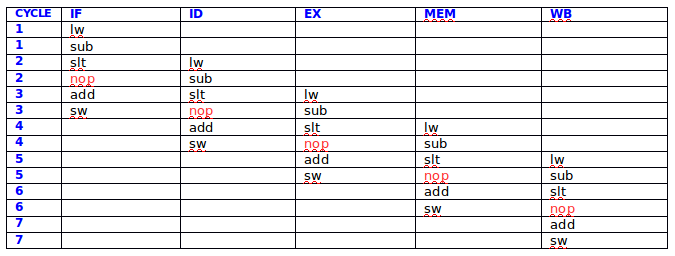
\includegraphics[width=1.1\textwidth]{hw7_p4a.png}
\end{figure}

\section*{4b)}


%%%%%%%%%%%%%%%%%%%%%%%%%%%%%%%%%%%%%%%%%%%%%%%%%%%%%%%%%%


\end{document}
